\section{Software Architecture}
This chapter describes the architecture of the software developed. First there will be a description of the big picture separating the software into several parts. Each of those parts will then be explained in greater detail in a seperate chapter.
\\\\
The software architecture has to fulfil multiple requirements for this project. It should be easily extendable with new algorithms and \acrshort{acro:UI} extensions. The input and output format of the application should be independent from the algorithms to support different file types like bitmap images or \gls{gloss:DXF}/\gls{gloss:DWG} formats. The algorithms of the application should be linked together as workflows which then can be executed by an engine simultaniously.

\begin{figure}[h]
  \centering
      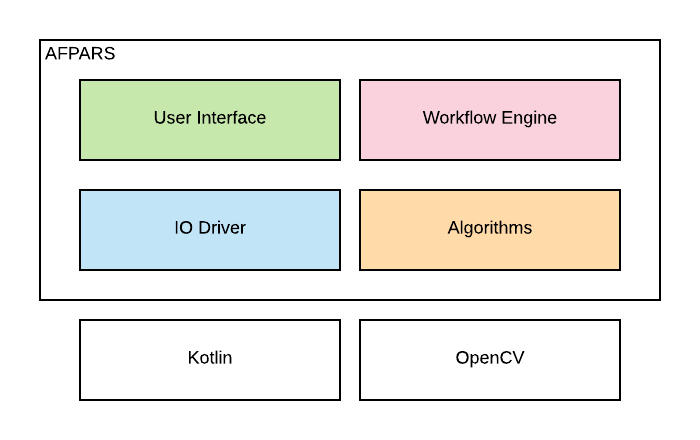
\includegraphics[width=1\textwidth]{AFPARS_Architecture}
  \caption{AFPARS software architecture.}
  \label{fig:AFPARS_Architecture}
\end{figure}


To fulfil these requirements, the architecture of the software is split into four parts as shown in Figure \ref{fig:AFPARS_Architecture}. The complete application is based on the \acrfull{acro:JVM} where \gls{gloss:Kotlin} is running on. For image processing and recognition the application uses the library \gls{gloss:OpenCV}.

\todo{What else should I write? Explain why it is important that the algorithm is easily interchangeable and why we did seperate those parts specifically. Why did we choose that sort of architecture over a different one. There is no mention of what holds all of this together ie. the workflow.}

\pagebreak

\subsection{Input / Output}
To support the different input and output formats the architecture uses a meta format for the
floor plan images called AFImage. Different \gls{gloss:Drivers} \todo{Define drivers in the glossary} add the support for multiple file formats. With this architecture it is possible to extend the software with new file formats and work internally with the meta container.

\begin{figure}[h]
  \centering
      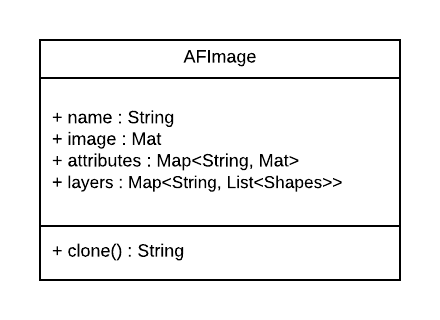
\includegraphics[width=0.6\textwidth]{AFImage_CD}
  \caption{AFImage class diagram.}
  \label{fig:AFImage_CD}
\end{figure}

The meta container AFImage contains a map of attributes (see Figure \ref{fig:AFImage_CD}) which can be used by algorithms to get information created by other algorithms or to store information into an existing image.

\todo{DWG / DXF Discussion}

\subsection{Algorithm}
\todo{rewrite, this is nonsense}
\todo{Explain why it is of importance that algorithms can be used in a pipeline and in different orders, why it is essential that we can swap them out, reuse them etx.}
To reuse algorithms in different workflows, the software architecture splits the algorithms into small parts which then can be connected together to pipelines. The algorithm itself does not know in which context it is running. As input parameter it gets just an AFImage from the last algorithm output and is able to return an AFImage again (see Figure \ref{fig:IAlgorithm_CD}). 

\begin{figure}[h]
  \centering
      \includegraphics[width=0.6\textwidth]{IAlgorithm_CD}
  \caption{Algorithm interface class diagram.}
  \label{fig:IAlgorithm_CD}
\end{figure}

\subsubsection{Parameter}
Because a lot of the algorithms need parameters to be set manually, there is the possibility to flag these parameters with an attribute in the code and the software is then able to automatically show a slider in the user interface. With this slider the user is able to set the parameter or use the default values (See Figure \ref{fig:parameter_window}).


\begin{figure}[h]
  \centering
      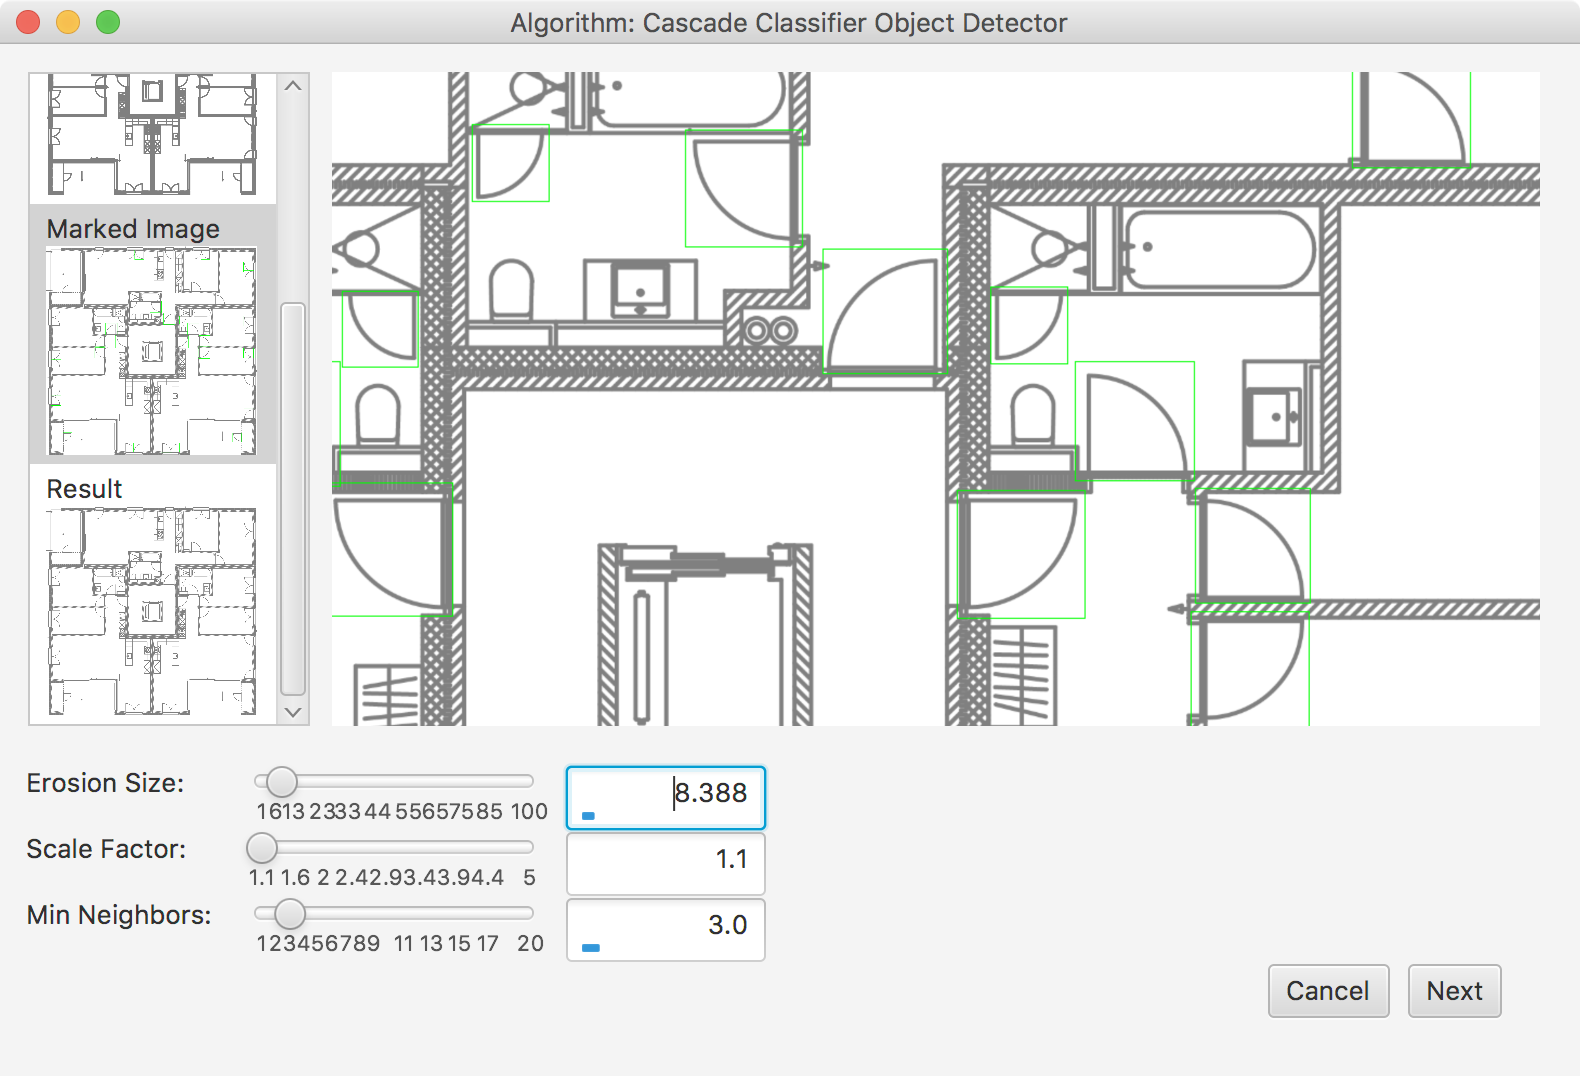
\includegraphics[width=0.6\textwidth]{parameter_window}
  \caption{Flag based parameter window.}
  \label{fig:parameter_window}
\end{figure}

\subsubsection{History}
As seen in Figure \ref{fig:IAlgorithm_CD} and Figure \ref{fig:parameter_window}, an algorithm is not just able to return one AFImage, instead it can return an unlimited count of AFImages, which then are displayed in the parameter window. These images are used to show a history of the steps the algorithm performed. This makes it easier to set the right parameter for the given algorithm and helps to debug all steps of an algorithm.

\subsection{Workflow}


\begin{figure}[h]
  \centering
      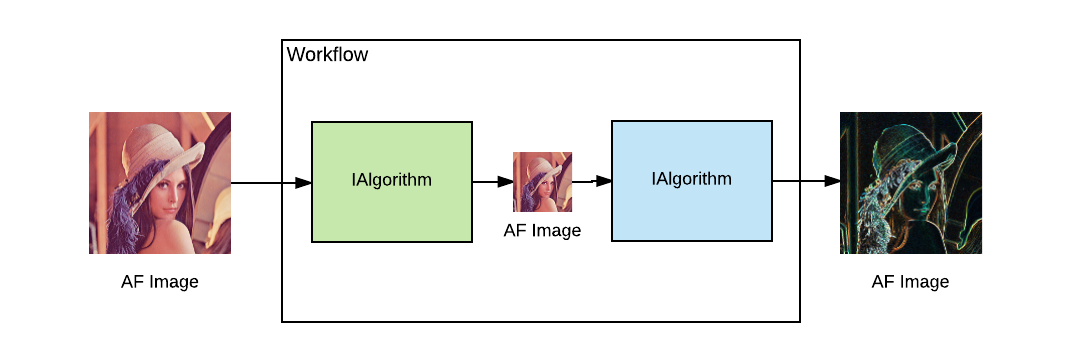
\includegraphics[width=1\textwidth]{workflow}
  \caption{Workflow example with two algorithms.}
  \label{fig:Workflow}
\end{figure}

\subsection{User Interface}
\missingfigure{User Interface Image.}
\todo{Why it looks like that. (Andere Software)}